\section{An\'alisis te\'orico del circuito}

A continuaci\'on se muestra una imagen del modelo del circuito considerando que los capacitores representan circuitos abiertos, ya que en este caso se trabaja con la señal continua, el mismo se esquematiza con el cálculo del equivalente de thevenin ya realizado entre el nodo de base y tierra.

	\subsection{Polarizaci\'on}
		
		\begin{figure}[H]
			\centering
			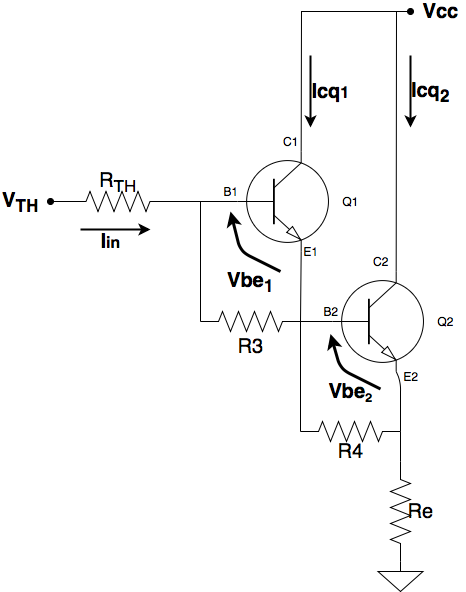
\includegraphics[scale=0.4]{./Imagenes/polarizacion.png} \\
			\caption{Circuito equivalente para el an\'alisis de polarizaci\'on.}
			\label{polarizacion}
		\end{figure}

Si se realiza el modelo equivalente de thevenin para los nodos de base y tierra.\\

		$
		\begin{cases}
		&V_{TH} = \frac{R_2}{R_1 + R_2} V_{CC}\\ \\
		&R_{TH} = R_1 // R_2 
		\end{cases}
		\label{Thevenin}
		$\\

A continuación se muestran las ecuaciones correspondientes al análisis de la malla de entrada, el transistor 2, el transistor 1 y el nodo conectado a la base del 2do transistor\\

		$
		\begin{cases}
		ME) \, \, V_{th}-I_{B1}R_{th}-V_{BEon_{1}}-V_{BEon_{2}}-R_{e}(I_{E_{2}}+I_{R_{4}})=0 \\  \\
		Q_{2}) I_{E_{2}}=I_{B_{2}}(\beta_{2}+1)\\ \\
		Q_{1}) \, \, I_{E_{1}} = I_{B_{1}}(\beta_{1}+1)\\ \\
		Nodo) \, \, I_{B_{2}} = I_{E_{1}} - \frac{V_{BEon_{2}}}{R_{4}}
		\end{cases}
		$\\

Con ellas ecuaciones, resolviendo podremos llegar a las siguientes expresiones para las corrientes de colector de ambos transistores.\\

		$
		\begin{cases}
		I_{cq_{1}}=\frac{V_{th}-V_{BEon_{1}}-V_{BEon_{2}}\left(1-\frac{R_{e}\beta_{2}}{R_{4}}\right)}{\frac{R_{th}}{\beta_{1}}+R_{e}\beta_{2}}\\ \\
		I_{cq_{2}}=V_{th}\frac{1}{\frac{R_{th}}{\beta_{1}\beta_{2}}+R_{e}\frac{\beta_{2}+1}{\beta_{2}}}-V_{BEon_{1}}\frac{1}{\frac{R_{th}}{\beta_{2}}+R_{e}\beta_{1}}-V_{BEon_{2}}\left(\frac{\beta_{2}}{R_{4}}+\frac{\left(1-\frac{R_{e}\beta_{2}}{R_{4}}\right)\cdot(\beta_{1}+1)}{\frac{R_{th}}{\beta_{2}}+R_{e}\beta_{1}} \right)
		\end{cases}
		$\\

Así recorriendo la malla de salida podremos ver que obtenemos las siguientes ecuaciones.\\

		$
		\begin{cases}
		V_{CEQ_{1}}=V_{CC}-V_{BEon_{2}}\left(1+\frac{R_{e}}{R_{4}}\right)-R_{e}I_{CQ_{2}}\\ \\
		V_{CEQ_{2}}=V_{CC}-V_{BEon_{2}}\frac{R_{e}}{R_{4}}-R_{e}I_{CQ_{2}}
		\end{cases}
		$\\
	

	\subsection{Modelo incremental}
	
	Tenemos que para cada transistor los estimadores tomados son los que se detallan a continuación.


		\begin{equation}
			\begin{cases}
			\widehat{r_{e}}=\frac{V_{T}}{I_{CQ}}\\
			\widehat{h_{ie}}=(\beta_{i}+1)R_{e_{i}}\\	
			\widehat{gm}=\frac{1}{R_{E}}
			\end{cases}
			\label{mod_inc_ecs}
		\end{equation}
	
	De esta forma, para el transistor $Q1$ se emplean las ecuaciones \ref{mod_inc_ecs} reemplazando i por 1, mientras que para el transistor $Q2$ se reemplaza i por 2. Así se obtienen los siguientes valores:
	
	\todo{COMPLETAR TABLA de estimadores}
	\begin{table}[h!]
		\centering
		\begin{tabular}{c c c}%
			\bfseries Estimadores & Q1 & Q2 \\ \hline
			$\widehat{g}_m$ &  & \\
			$\widehat{h}_{ie}$ &  & \\
			$\widehat{r}_{ce}$&  & \\
			\hline
		\end{tabular}
		\caption{Estimadores correspondientes al modelo incremental, para los transistores Q1 y Q2.}
		\label{avolf}
	\end{table}
	
	\subsection{Circuito incremental}
	
		
		\begin{figure}[H]
			\centering
			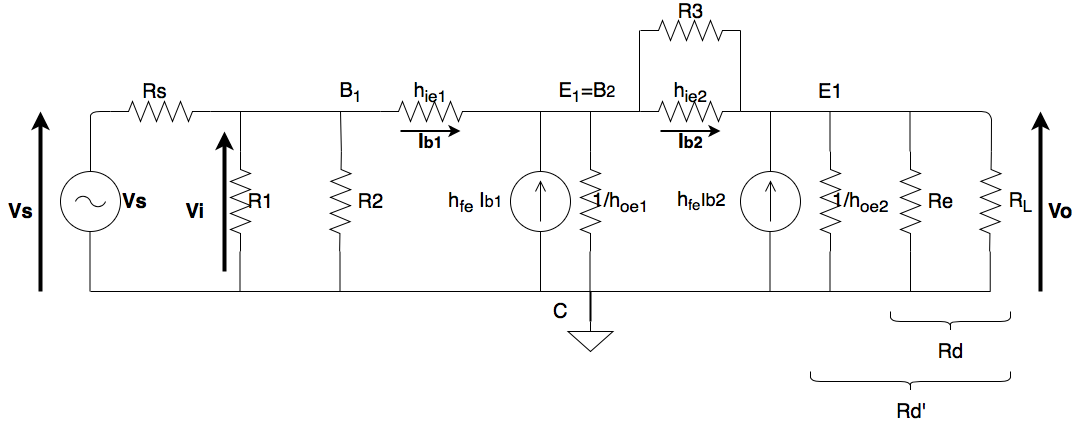
\includegraphics[scale=0.4]{./Imagenes/circ_incremental.png} \\
			\caption{Circuito equivalente para el an\'alisis del circuito incremental.}
			\label{circ_incremental}
		\end{figure}

A continuacion se muestran las ecuaciones que rigen las reducciones del circuito para facilitar su análisis, las mismas incluyen paralelos de resisitencias y pasaje a nivel de corriente. \\

		$
		\begin{cases}
		hfe_{2}^{*}=hfe_{2}\frac{R_{4}}{R_{4}+hie_{2}} \\
		hie_{2}^{*}=hie_{2}//R_{4} \\
		R_{d}=R_{e}//R_{2}
		\end{cases}
		\label{mod_inc_ecs}
		$ \\

De esta manera las expresiones para las impedancias que se ven a la entrada del primer transistor, del amplificador y del sistema se muestran a continuación. \\

		$
		\begin{cases}	
		R_{i}=hie_{1}+(hfe_{1}+1)hie_{2}^{*}+(hfe_{2}^{*}+1)(hfe_{1}+1)R_{d} \\
		R_{ia}=R_{i} // R_{th} \\
		R_{is}=R_{s}+R_{ia}
		\end{cases}
		\label{mod_inc_ecs}
		$\\

A continuación se muestran dos expresiones halladas que servirán de base para luego facilitar el cálculo de la ganancia del sistema.\\

		$
		\begin{cases}	
		\frac{V_{o}}{ib_{2}}=R_{d}(hfe_{2}^{*}+1) \\
		\frac{V_{i}}{V_{s}}=\frac{R_{ia}}{R_{ia}+R_{s}}
		\end{cases}
		\label{mod_inc_ecs}
		$\\

Así la ecuación de la ganancia en tensión del sistema se puede expresar de la siguiente forma. \\

	\begin{equation}	
		\Delta _{vs}=\frac{V_{o}}{V_{s}}=\frac{V_{o}}{ib_{2}}\cdot\frac{ib_{2}}{ib_{1}}\cdot\frac{ib_{1}}{V_{i}}\cdot\frac{V_{i}}{V_{s}}=R_{d}(hfe_{2}^{*}+1)(hfe_{1}+1)\frac{1}{R_{i}}\frac{Ria}{Ria+Rs}
		\label{mod_inc_ecs}
	\end{equation}

La ganancia de corriente la podremos expresar como \\

	\begin{equation}	
		\Delta _{i}=\frac{I_{Rd}}{ib_{1}}=(hfe_{2}^{*}+1)(hfe_{1}+1)
		\label{mod_inc_ecs}
	\end{equation}

	\begin{equation}	
	\Delta_{is}=\frac{I_{Rd}}{I_{Rs}}\cdot\frac{I_{b_{1}}}{I_{Rs}}=\Delta_{i}\frac{R_{th}}{R_{th}+R_{i}}
	\label{mod_inc_ecs}
	\end{equation}

	\begin{equation}	
		\Delta_{is}^{\, \, \,'}=\frac{I_{Rl}}{I_{Rs}}=\frac{I_{Rl}}{I_{Rd}}\cdot\frac{I_{Rd}}{I_{Rs}}=\frac{R_{e}}{R_{e}+R_{2}}\Delta_{is}
		\label{mod_inc_ecs}
	\end{equation}

Donde $\Delta_{i}$ es la ganancia de corriente, $\Delta_{is}$ es la ganancia de corriente del sistema y $\Delta_{is}^{\, \, \,'}$ es la ganancia de corriente del sistema sobre la carga.
\section{Diseño del circuito}